\section{Finanzen}
\autorbeginn{Marcel}
\label{sec:ui-bank}

Eine zentrale Informationsquelle des Spielers zeigt die Benutzeroberfläche „Finanzen". Hier erhält der Spieler eine Übersicht über alle im Unternehmen durchgeführten Geldflüsse. Die Benutzeroberfläche ist in drei zentrale Elemente untergliedert. Es handelt sich um die Einnahmen und Ausgaben pro Spielrunde sowie einen kurzen Überblick über die gesamte Geldsituation in dem Unternehmen.
 
Die Einnahmen pro Spielrunde werden den Ausgaben pro Spielrunde gegenübergestellt und befinden sich im linken Teil der Benutzeroberfläche. Das Unternehmensplanspiel Star Greg ist darauf ausgerichtet, ausschließlich Raumschiffe zu produzieren. Deshalb besteht der Umsatz des Unternehmens lediglich aus den Preisen des jeweiligen Raumschiffs multipliziert mit der verkauften Anzahl. Daraus folgt, dass es insgesamt drei Einnahmequellen gibt. Es handelt sich um den Umsatz des X Wings, der Correllian Corvette und den Umsatz des Millenium Falken. Diese drei verschiedenen Umsätze werden in einer einfachen Tabelle dargestellt und aufsummiert. Die Gesamteinnahmen der Spielrunde werden dem Spieler in einem grün hinterlegten Textfeld unterhalb der drei Einnahmequellen angezeigt.
 
Neben den Einnahmen gibt es Ausgaben pro Spielrunde. Diese werden im rechten Teil der Benutzeroberfläche dargestellt. Die Ausgaben fallen in drei Bereichen des Unternehmens an. Es handelt sich um die Produktion, das Lager und das Personal. Die Ausgaben der Produktion setzen sich aus fünf Posten zusammen. Es sind Gesamtkosten für alle gekauften Triebwerke, Hitzeschilder, Rumpfbauteile und Sonderbauteile. Zusätzlich werden zu den Produktionskosten auch die durch den Ausschuss verursachten  Zusatzkosten hinzugerechnet. Unterhalb der Produktionskosten werden die Personalkosten aufgelistet. Diese setzen sich aus den Werbungskosten, laufenden Kosten (Wartungskosten), und den Kosten der Umbaumaßnahmen zusammen. Das dritte Element der Ausgaben pro Spielrunde sind die gesamten Lagerkosten. Sie setzen sich aus den belegten Lagerplatzeinheiten multipliziert mit den Kosten pro Lagerplatzeinheit zusammen.
 
Die gesamten Ausgaben pro Spielrunde werden in einem rot hinterlegten Textfeld dargestellt. Durch das grün hinterlegte Textfeld der Einnahmen pro Spielrunde und das rot hinterlegte Textfeld der Ausgaben pro Spielrunde soll der Spieler schon bei kurzer Betrachtung des Bildschirms einen Überblick über die Geldflüsse im Unternehmen bekommen.
  
Im unteren Teil der Benutzeroberfläche befindet sich ein Überblick über die gesamte Finanzsituation im Unternehmen. In der ersten Zeile der Tabelle wird der Kontostand zu beginn der Spielrunde angezeigt. Darunter befinden sich die Ein- und Ausgaben der Spielrunde sowie der Kontostand am Ende der Spielrunde(s. \ref{img:ui-bank}).

\begin{figure}[htb]
  \centering
  \fbox{
    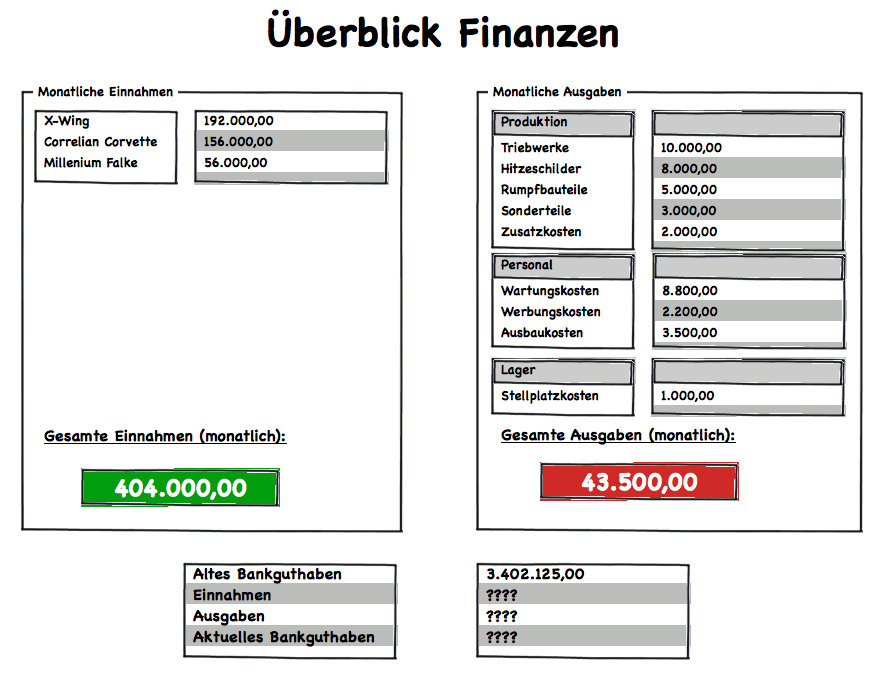
\includegraphics[width=0.9\textwidth]{40_UI/30_Bank/Bank.jpg}
  }
  \caption{Finanzen}
  \label{img:ui-bank}
\end{figure}


\autorende{}